\documentclass[3p,times,procedia]{elsarticle}
\flushbottom
\usepackage{ecrc}
\usepackage[bookmarks=false]{hyperref}
\hypersetup{colorlinks,linkcolor=blue,citecolor=blue,urlcolor=blue}
\volume{00}
\firstpage{1}
\journalname{Procedia Computer Science}
\runauth{Daoud et al.}
\jid{procs}
\usepackage{amssymb}
\usepackage{amsmath}
\usepackage{booktabs}
\usepackage{graphicx}
\usepackage{array}
\usepackage{url}
\graphicspath{{./}{figs/}}
\setlength{\emergencystretch}{3em}
\setlength{\textfloatsep}{3pt plus 1pt minus 1pt}
\setlength{\floatsep}{3pt plus 1pt minus 1pt}
\setlength{\intextsep}{3pt plus 1pt minus 1pt}
\setlength{\abovecaptionskip}{3pt}
\setlength{\belowcaptionskip}{0pt}
\begin{document}
\begin{frontmatter}
\dochead{The 18th International Conference on Ambient Systems, Networks and Technologies (ANT) \\ April 13-15, 2027, Delft, the Netherlands}
\title{Demand shift robustness of learned fleet rebalancing on NYC ride-hailing data}
\author[a]{Alaa Daoud}
\author[c]{Srinivasa K G}
\author[b]{Avani Dewangan}
\author[b]{Md Athar Sharif\corref{cor1}}
\author[b]{Prashil Thul}
\address[a]{LAMIH, CNRS UMR 8201, INSA Hauts-de-France, Universit\'e Polytechnique Hauts-de-France, Valenciennes, France}
\address[b]{Department of Computer Science and Engineering, IIIT Naya Raipur, Naya Raipur, India}
\address[c]{Department of Data Science and Artificial Intelligence, IIIT Naya Raipur, Naya Raipur, India}
\begin{abstract}
We measure how frozen multi-agent rebalancing policies degrade when deployment demand departs from training demand, and what closes the gap to a tuned rolling-horizon linear program (LP). On NYC16, a sixteen-zone Manhattan network built from TLC trip records, we evaluate IPPO, MAPPO and a greedy dispatcher against the LP on two held-out temporal splits and eight synthetic shifts grouped into temporal, volume/burst and spatial families, using twelve paired windows and five training seeds. Every service gain is reported together with the empty distance it cost. MAPPO serves more than IPPO in every scenario on paired windows ($+3.08$~pp at base, $p=3.3\times10^{-3}$), but both trail the LP ($71.0\%$ at $295$~km). We trace the gap to three mechanisms: optimisation rather than capacity (behaviour cloning the LP into the same network reaches $70.3\%$), argmax symmetry breaking (sampled actions recover $+4.6$ to $+7.9$~pp at higher distance), and relocation legs $50\%$ longer than the LP's. A $2\times2$ study of permutation-equivariant zone attention and domain randomisation shows that only the combination works: it reaches $69.1\%$ at $393$~km at base, matches the LP on the test split ($71.0\%$ vs $71.8\%$) and on zone permutation, and exceeds it under $60\%$ single-zone concentration ($51.2\%$ vs $48.4\%$, $+16.3$~pp over MLP-MAPPO). Spatial-family retention rises to $83.8\%$, against $80.7\%$ for the LP (not significant). Either component alone does not help.
\end{abstract}
\begin{keyword}
fleet rebalancing; multi-agent reinforcement learning; MAPPO; IPPO; dynamic dispatch; linear programming; demand shift
\end{keyword}
\cortext[cor1]{Corresponding author. }
\end{frontmatter}
\email{md24100@iiitnr.edu.in}

\section{Introduction}
\label{sec:intro}

A rebalancing policy is judged on two numbers: the share of orders it serves and the distance its vehicles drive empty. They trade against each other almost freely, since relocating vehicles buys service with distance, so we never report one without the other. Ride-hailing demand moves with seasons, events and new hotspots, and retraining daily is expensive, so what matters in deployment is how a frozen policy behaves on demand it did not train on.

We ask four questions on a network built from recorded demand. RQ1: how much does performance degrade under temporal, volume and spatial shifts? RQ2: do independent (IPPO) and shared-critic (MAPPO) learners degrade differently? RQ3: how do they compare with a tuned LP rebalancer, and why? RQ4: can architectural symmetry and training-time randomisation close the gap under spatial shift? This is a measurement study with a targeted mitigation; we do not claim a new algorithm. Contributions: (i) a reconciled reward and a paired twelve-window protocol, (ii) a diagnosis of the learned-to-LP gap into three mechanisms, and (iii) a $2\times2$ ablation showing that permutation equivariance and domain randomisation are each insufficient and jointly effective.

\section{Related work}
\label{sec:related}

Reinforcement learning entered ride-hailing through order dispatch: learned values with combinatorial planning~\cite{xu2018}, cooperative agents on a hexagon grid~\cite{lin2018} and a deployed policy at DiDi~\cite{qin2020}. Repositioning asks where supply should be before the order appears, and has its own literature: model-free fleet management~\cite{oda2018}, distributed deep RL~\cite{alabbasi2019}, joint dispatching and repositioning~\cite{holler2019}, mean-field MARL~\cite{li2019}, reward design~\cite{shou2020}, a real-world deployment~\cite{jiao2021} and graph-based rebalancing~\cite{gammelli2021}. Our LP descends from the matching-integrated rolling-horizon model of Guo~\emph{et al.}~\cite{guo2021}. We use PPO~\cite{schulman2017} in a PettingZoo AEC environment~\cite{pettingzoo}, in the IPPO and MAPPO forms of Yu~\emph{et al.}~\cite{yu2022}. For robustness we follow the freeze-perturb-report discipline of robust adversarial RL~\cite{pinto2017} and domain randomisation~\cite{tobin2017}, within the generalisation framing of Kirk~\emph{et al.}~\cite{kirk2023}. The equivariant encoder uses scaled dot-product attention~\cite{vaswani2017}, which is permutation-equivariant over set elements~\cite{zaheer2017} once positional identity is removed, the same motivation as graph-based rebalancing~\cite{gammelli2021}. Value decomposition~\cite{rashid2018}, counterfactual credit~\cite{foerster2018} and continuous-action or mean-field methods~\cite{lowe2017,yang2018} are left to future work.

\section{Environment and protocol}
\label{sec:env}

\subsection{Network, demand and fleet}
\label{sec:network}

NYC16 keeps the sixteen taxi zones with the highest volume in the April 2026 High Volume For-Hire Vehicle records~\cite{tlc2026} (IDs 68, 79, 112, 145, 161, 162, 163, 164, 170, 230, 231, 234, 236, 237, 246, 249) and snaps their centroids to a Manhattan road graph of 4{,}861 nodes and 10{,}457 edges. We draw 108 hourly windows from 6--14 April 2026, split in time into 84 training, 12 validation (13 April) and 12 test windows (14 April). An episode plays one window, capped at 130 orders, with 26 vehicles at 30~km/h, lasting 60~min in 0.5~min steps; an order that waits 5~min cancels (Table~\ref{tab:params}).

\subsection{Markov decision process}
\label{sec:mdp}

The problem is a cooperative multi-agent MDP with discount $\gamma=0.99$, stepped zone by zone in AEC order. Each zone controller chooses one of 33 discrete actions: $0$ is no-op; $1..16$ dispatch pending candidate order $0..15$ within the 2~km radius; $17..32$ relocate one idle driver to target zone $0..15$, masked to legal targets. The 615-dimensional observation holds zone location (2), own state (4), all-zone state ($16\times4$), pending orders ($16\times6$), pending mask and passengers ($2\times16$), neighbour mask (16), a 24-step demand history per zone ($16\times24$), elapsed fraction (1) and inbound fleet share (16), normalised by a running maximum within the episode. The MAPPO critic additionally receives the 593-dimensional global state.

\subsection{Reconciled objective}
\label{sec:objective}

The team reward per episode is
\begin{equation}
  R = \omega\, n_{\mathrm{served}} - \beta\, d_{\mathrm{empty}} - \alpha\, W_{\mathrm{acc}} - c\, n_{\mathrm{cancel}},
  \qquad
  W_{\mathrm{acc}} = \frac{1}{\tau}\sum_{t}\sum_{z}\sum_{o\in P_z(t)} w_o(t),
  \label{eq:objective}
\end{equation}
with $\omega=1.0$, $\beta=0.06$ per empty km, $\alpha=0.2$, $c=1.0$ and patience $\tau=5$~min. Here $w_o(t)$ is measured in minutes, so $w_o(t)/\tau$ is dimensionless; $W_{\mathrm{acc}}$ accumulates the wait of every order pending in zone $z$ at turn $t$, normalised by patience. Across all 9{,}684 evaluated episodes (4{,}224 baseline/ablation + 5{,}460 mitigation) the environment reward matches Eq.~\eqref{eq:objective} within $6.09\times10^{-6}$, and the empty-distance attribution $d_{\mathrm{empty}} = d_{\mathrm{reloc}} + d_{\mathrm{pickup}}$ holds to $1.71\times10^{-12}$~km, so reward and KPIs below are mutually consistent.

\begin{table}[tbp]
\centering
\caption{NYC16 environment and training configuration.}
\label{tab:params}
\footnotesize
\begin{tabular}{lr@{\hspace{2.2em}}lr}
\toprule
Parameter & Value & Parameter & Value \\
\midrule
Zones / road nodes / edges & 16 / 4{,}861 / 10{,}457 & $\omega$, $\beta$, $\alpha$, $c$ & 1.0, 0.06, 0.2, 1.0 \\
Windows (train/val/test) & 84 / 12 / 12 & Patience $\tau$ & 5 min \\
Vehicles, speed & 26, 30 km/h & Discount $\gamma$ & 0.99 \\
Order cap per window & 130 & PPO $\epsilon$, entropy, GAE $\lambda$ & 0.2, 0.01, 0.99 \\
Episode / step & 60 / 0.5 min & PPO epochs, lr, grad clip & 4, $3\times10^{-4}$, 0.5 \\
Actions / obs.\ dim & 33 / 615 & Iterations, seeds & 200, 5 \\
\bottomrule
\end{tabular}
\end{table}

\subsection{Baselines, learners and evaluation}
\label{sec:baselines}

\textbf{Greedy} assigns each order to the nearest idle vehicle and never relocates. \textbf{LP} is a rolling-horizon transportation programme solving matching and rebalancing jointly each turn with an exponential moving-average forecast; its lookahead and deficit penalty were grid-tuned on training windows only, giving lookahead $5.0$ and deficit penalty $1.0$. \textbf{IPPO} and \textbf{MLP-MAPPO} share one actor (Linear 615$\to$256--Tanh--256$\to$256--Tanh, 33-way masked head) across the homogeneous zones; MAPPO adds a separate centralised critic. Both are trained for 200 iterations of PPO with five seeds, and the final iterate (it200) is reported.

Evaluation steps zones sequentially over 12 paired windows (seeds 1000--1011) per scenario. S3 covers each validation window once and S6 each test window once; training-split scenarios draw 12 paired episodes with replacement from the 84 training windows, yielding 10 unique windows (4, 17, 24, 29, 36, 43, 50, 58, 61, 75) identically across every arm. Actions are argmax unless marked sampled. Standard deviations use ddof${}=1$ across five seeds for learned arms and across the 12 windows for the deterministic baselines. Comparisons use paired per-window $t$-tests and Wilcoxon signed-rank tests on the $n=12$ window means.

\subsection{Shift scenarios}
\label{sec:taxonomy}

We group scenarios into three families and never pool across them, since under-loading (S2a) yields retention above $100\%$. Divergence from training demand is total variation (TV) and Jensen--Shannon (JSD, bits) over zone shares. \emph{Temporal}: S3 (validation split; TV $0.204$, JSD $0.052$) and S6 (test split; TV $0.220$, JSD $0.057$). \emph{Volume/burst}: S2a, S2b, S2d, S2e scale the order cap by $0.5$, $0.75$, $1.5$, $2.0$; S5 redirects $20\%$ of orders in minutes 20--30 to zone 0 (taxi zone 68; TV $0.035$). \emph{Spatial}: S1 rotates zone identities by offset 8 with probability $p=1.0$ (TV $0.254$, JSD $0.071$); S4 sends $60\%$ of demand to zone 1 (taxi zone 79; TV $0.563$, JSD $0.310$); S7 drifts a hotspot from zone 12 to zone 10 (TV $0.044$). Parametric sweeps vary $p\in\{0,0.25,0.5,0.75,1.0\}$ in S1 and the zone-1 share in $\{10,20,40,60,80\}\%$ in S4, plus S4 at $60\%$ in the coldest zone (index 5, taxi zone 162, $4.84\%$ of training demand).

\section{Base condition and IPPO versus MAPPO}
\label{sec:results}

Table~\ref{tab:s0} and Fig.~\ref{fig:pareto} give the base condition. The LP serves $71.0\%$ with $294.8$~km empty, of which $202.2$~km are relocation legs ($1.72$~km of relocation per move; total empty distance is $2.51$~km per move). MLP-MAPPO serves $64.3\%$ with $398.7$~km and IPPO $61.3\%$ with $375.6$~km; greedy serves $44.9\%$ on pickup travel alone. Both learners are dominated by the LP on both axes and on reward ($+8.7$ for LP against $-21.7$ and $-33.2$).

\textbf{RQ2.} On paired windows MLP-MAPPO serves more than IPPO in every scenario: S0 $+3.08\pm2.86$~pp (paired $t$ $p=3.34\times10^{-3}$, Wilcoxon $p=4.88\times10^{-3}$), S1 $+2.53$~pp ($p=0.011$), S4 $+6.12$~pp ($p=2.11\times10^{-5}$), S6 $+2.65$~pp ($p=1.01\times10^{-3}$). A Welch test across the five seeds does not detect the S0 difference ($p=0.15$); an earlier version of this study used that seed-level test on five episodes and concluded that the two were indistinguishable, which the paired protocol overturns. IPPO's weakness is seed-level collapse: its empty-distance spread is $\pm91.3$~km at S0 and $\pm274.8$~km at S4, and its best checkpoint ($64.1\%$) sits well above the final iterate ($61.3\%$). The centralised critic therefore matters here mainly as a stabiliser.

\begin{table}[tbp]
\centering
\caption{Base condition (S0), 12 paired windows. Learned arms: mean $\pm$ std across five seeds (argmax unless marked); baselines: $\pm$ across windows.}
\label{tab:s0}
\scriptsize
\setlength{\tabcolsep}{2.0pt}
\begin{tabular}{lcccccc}
\toprule
Method & SR (\%) & Empty km & Reloc / pickup km & Relocations & Wait (min) & $R$ \\
\midrule
Greedy             & 44.9 $\pm$ 8.6 & 68.9 $\pm$ 13.8  & 0.0 / 68.9   & 0.0             & 2.36 $\pm$ 0.22 & $-80.7 \pm 28.3$ \\
LP                 & 71.0 $\pm$ 4.4 & 294.8 $\pm$ 15.3 & 202.2 / 92.6 & 117.7 $\pm$ 8.2  & 2.58 $\pm$ 0.21 & $+8.7 \pm 11.9$ \\
IPPO-it200         & 61.3 $\pm$ 3.8 & 375.6 $\pm$ 91.3 & 287.2 / 88.4 & 116.9 $\pm$ 34.5 & 2.58 $\pm$ 0.19 & $-33.2 \pm 11.4$ \\
MLP-MAPPO          & 64.3 $\pm$ 1.7 & 398.7 $\pm$ 46.1 & 304.2 / 94.5 & 125.9 $\pm$ 22.1 & 2.65 $\pm$ 0.14 & $-21.7 \pm 4.6$ \\
\midrule
IPPO sampled       & 69.2 $\pm$ 0.7 & 447.1 $\pm$ 22.4 & 347.0 / 100.2 & 146.0 $\pm$ 4.1 & 2.60 $\pm$ 0.05 & $-4.3 \pm 2.3$ \\
MAPPO sampled      & 68.9 $\pm$ 1.3 & 451.0 $\pm$ 10.6 & 350.6 / 100.3 & 142.9 $\pm$ 8.1 & 2.58 $\pm$ 0.09 & $-5.0 \pm 4.5$ \\
BC-LP-rw10         & 70.3 $\pm$ 3.9 & 358.1 $\pm$ 25.4 & 263.8 / 94.4 & 148.2 $\pm$ 12.1 & 2.55 $\pm$ 0.22 & $+4.8 \pm 15.0$ \\
\midrule
Attention-MAPPO    & 64.4 $\pm$ 1.9 & 259.4 $\pm$ 40.6 & 166.3 / 93.1 & 94.2 $\pm$ 20.0 & 2.75 $\pm$ 0.11 & $-14.4 \pm 6.5$ \\
DR-MLP-MAPPO       & 65.4 $\pm$ 1.5 & 475.7 $\pm$ 9.9  & 386.6 / 89.2 & 155.8 $\pm$ 11.4 & 2.41 $\pm$ 0.09 & $-21.5 \pm 6.4$ \\
DR-Attention-MAPPO & 69.1 $\pm$ 1.5 & 393.0 $\pm$ 26.8 & 295.7 / 97.3 & 138.8 $\pm$ 21.0 & 2.72 $\pm$ 0.08 & $-3.8 \pm 6.2$ \\
\bottomrule
\end{tabular}
\end{table}

\begin{figure}[tbp]
\centering
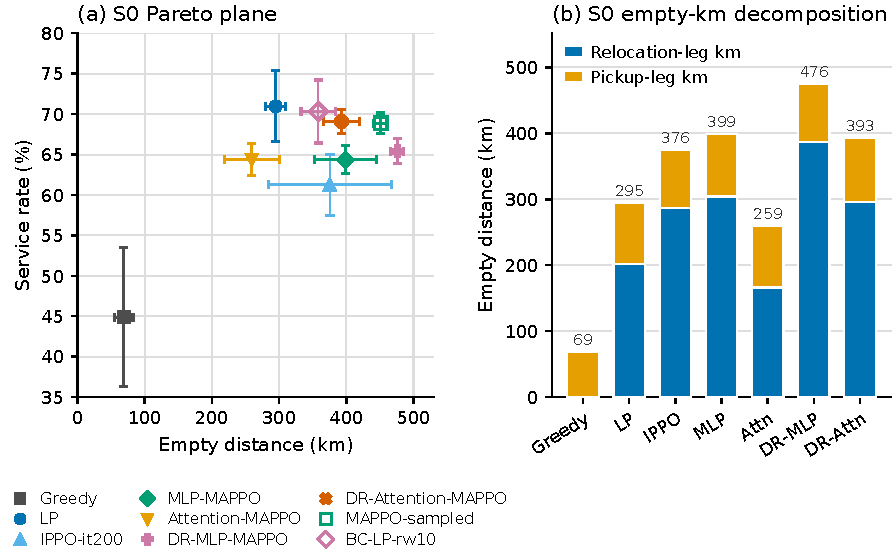
\includegraphics[width=0.73\textwidth]{fig1_pareto_and_decomp.pdf}
\caption{S0 on 12 paired windows. (a) Service rate against empty distance, $\pm1$ std (seeds for learned arms, windows for baselines). (b) Empty distance split into relocation legs and pickup legs.}
\label{fig:pareto}
\end{figure}

\section{Why vanilla learners trail the LP}
\label{sec:mechanisms}

\textbf{Optimisation, not capacity.} \emph{BC-LP-rw10} fits the identical $615\to256\to256\to33$ flat MLP by masked weighted cross-entropy on $116{,}160$ decisions from $60$ training episodes ($45/84$ distinct windows) generated by the tuned LP (20 epochs, batch $512$, Adam $10^{-3}$, grad clip $5.0$, $10\times$ weight on the $6.0\%$ relocation actions to prevent no-op collapse). It reaches $70.3\pm3.9\%$ at $358.1$~km and $R=+4.8$ on S0, $50.1\pm6.0\%$ at $312.0$~km on S4, and $71.2\pm3.8\%$ on S6; the $\pm3.9\%$, $\pm25.4$~km and $\pm15.0$ in $R$ are across the 12 paired evaluation windows of that single fit. The network can represent an LP-quality policy; PPO with per-zone credit does not find it.

\textbf{Symmetry breaking under argmax.} Sixteen controllers sharing one actor and seeing near-identical inputs take near-identical argmax actions. Evaluating it200 with sampled actions raises S0 service to $69.2\pm0.7\%$ for IPPO and $68.9\pm1.3\%$ for MAPPO, $+7.9$ and $+4.6$~pp over argmax, but at $447.1$ and $451.0$~km: sampling buys service with distance and is not a free fix.

\textbf{Relocation leg length and collapse.} MLP-MAPPO relocates about as often as the LP ($125.9$ vs $117.7$ moves) but drives $50\%$ more relocation distance ($304.2$ vs $202.2$~km; $2.42$ vs $1.72$~km of relocation per move, or $3.23$ vs $2.51$~km total empty per move), so it is choosing worse destinations, not moving more. Under S4 it drives $460.3$~km ($395.3$~km relocating) yet serves only $34.9\%$, while one seed freezes to minimal relocation.

\section{Degradation under demand shift}
\label{sec:shifts}

Fig.~\ref{fig:shifts} gives absolute service and empty distance per scenario. Temporal shifts barely move any policy: on the test split S6 the LP serves $71.8\%$ and the ranking at S0 is preserved. Volume and burst shifts degrade all arms similarly, with overload (S2e) compressing differences. Spatial shifts are where policies separate. Zone permutation (S1) costs $10.4$--$16.7$~pp across arms (LP $16.7$, MLP-MAPPO $13.6$, IPPO $13.1$, Greedy $10.4$), and single-zone concentration (S4) drops MLP-MAPPO to $34.9\%$ against $48.4\%$ for the LP. Fig.~\ref{fig:param} shows that both losses grow smoothly with the shift: the S1 sweep degrades monotonically in $p$ for the LP and all learned arms, and in the S4 sweep the vanilla learners fall faster than the LP as concentration rises, reaching $22.0\pm2.9\%$ (MLP-MAPPO) against $36.5\pm4.3\%$ (LP) at $80\%$. Concentrating $60\%$ of demand on the coldest zone gives the same pattern: MLP-MAPPO serves $36.2\%$ against $56.3\%$ for the LP. Since every NYC16 zone holds $4.84$--$8.29\%$ of training demand, S4 tests concentration on familiar zones, not unseen support.

\begin{figure}[tbp]
\centering
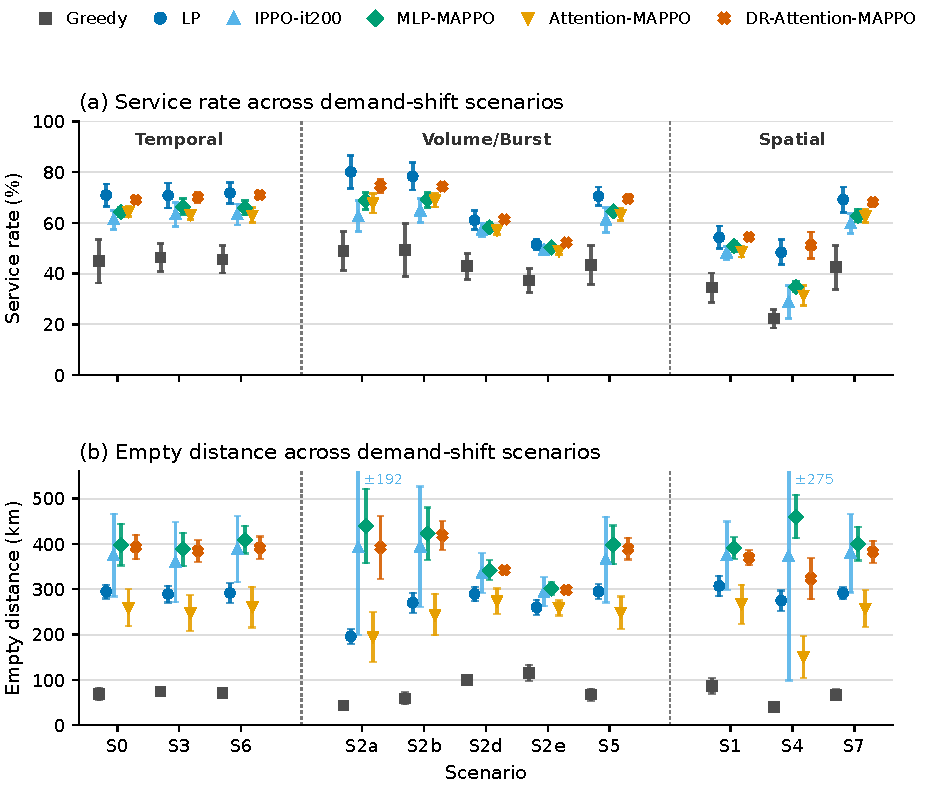
\includegraphics[width=0.57\textwidth]{fig2_shift_scenarios.pdf}
\caption{Service rate (a) and empty distance (b) per scenario, grouped by family; markers are means, ticks $\pm1$ std. Annotations mark IPPO's empty-distance spread where it leaves the axis. DR-MLP-MAPPO is omitted for readability and reported in Table~\ref{tab:shift} and Figs.~\ref{fig:param}--\ref{fig:retention}.}
\label{fig:shifts}
\end{figure}

\section{Mitigation: equivariance and domain randomisation}
\label{sec:planb}

The mechanisms above suggest two complementary fixes. Slot-indexed MLP inputs tie each zone's behaviour to its index, which spatial shifts break, and the training distribution never shows concentrated or permuted demand.

\textbf{Architecture and training.} The \emph{ZoneAttentionEncoder} attends over the sixteen zones~\cite{vaswani2017} and is permutation-equivariant~\cite{zaheer2017}: it has no zone-index embedding and produces relocation logits exclusively from an equivariant destination head, so permuting zones permutes the relocation distribution. With domain randomisation (DR), each training episode is base S0 with probability $0.34$, a random zone permutation applied with probability $p\sim U(0.5,1.0)$ with probability $0.33$, or a random single-zone concentration with share $U(20\%,75\%)$ with probability $0.33$~\cite{tobin2017}. DR is disabled in validation and evaluation. Crossing the two factors gives four MAPPO arms (Table~\ref{tab:shift}).

\begin{table}[tbp]
\centering
\caption{Cross-shift service rate (\%) for the $2\times2$ study, 12 paired windows, five seeds. S4 km and S6 km are empty distance under S4 and S6. Retention is family service relative to the arm's own S0. z1@80 and z5@60: S4 sweep at $80\%$ on zone 1 and $60\%$ on cold zone 5. Five-seed means (12-window means for LP); per-scenario standard deviations appear in Figs. 2--3.}
\label{tab:shift}
\scriptsize
\setlength{\tabcolsep}{2.0pt}
\begin{tabular}{lcccccccccccc}
\toprule
 & & & & & & & & & & \multicolumn{3}{c}{Retention (\%)} \\
\cmidrule(lr){11-13}
Method & S0 & S1 & S4 & S4 km & S6 & S6 km & S7 & z1@80 & z5@60 & Spatial & Vol./burst & Temporal \\
\midrule
LP                 & 71.0 & 54.3 & 48.4 & 274.9 & 71.8 & 291.8 & 69.2 & 36.5 & 56.3 & 80.7 & 96.3 & 100.5 \\
MLP-MAPPO          & 64.3 & 50.7 & 34.9 & 460.3 & 66.0 & 409.5 & 62.8 & 22.0 & 36.2 & 76.9 & 96.7 & 102.8 \\
Attention-MAPPO    & 64.4 & 48.7 & 31.4 & 150.4 & 62.9 & 260.5 & 62.6 & 20.4 & 34.2 & 73.9 & 95.0 & 98.0 \\
DR-MLP-MAPPO       & 65.4 & 51.6 & 35.2 & 542.1 & 67.2 & 471.9 & 62.8 & 25.0 & 56.9 & 76.2 & 96.8 & 103.0 \\
DR-Attention-MAPPO & \textbf{69.1} & \textbf{54.4} & \textbf{51.2} & 323.7 & \textbf{71.0} & 391.7 & \textbf{68.2} & \textbf{44.3} & 55.8 & \textbf{83.8} & 96.1 & 102.1 \\
\bottomrule
\end{tabular}
\end{table}

\textbf{Encoder and critic.} The encoder uses single-head scaled dot-product attention with $d_{\mathrm{emb}}=64$: \texttt{order\_embed} is $\mathrm{Linear}(7\to64)$--Tanh over pending orders, while \texttt{zone\_embed} is $\mathrm{Linear}(31\to64)$--Tanh over four zone scalars, 24 demand-history steps and relative centroid offsets $(dx,dy,\mathrm{dist})$ from \texttt{zone\_xy}; a learned scalar \texttt{neighbor\_bias} is added to legal-neighbour attention logits. The trunk maps $[\text{self\_ctx}(6),\text{order\_pool}(64),\text{zone\_pool}(64),\text{time\_frac}(1)]$ through $135\to256\to256$ with Tanh. Actions $0..16$ come from \texttt{actor(h)[:, :17]}; actions $17..32$ come exclusively from the equivariant destination head, summing $\langle\texttt{dest\_key}(\text{zone\_emb}_j),\texttt{self\_query}(\text{self\_ctx})\rangle/\sqrt{256}$ with $\texttt{dest\_key},\texttt{self\_query}:\mathbb{R}^{64}\to\mathbb{R}^{256}$, $\texttt{dest\_bias}(\text{all\_zone\_state}_j,\text{demand\_hist}_j,\text{inbound}_j)$, and $\texttt{travel\_cost}(dx_j,dy_j)+\texttt{dist\_cost}(10\cdot\mathrm{dist}_j)$. The attention module (actor plus local value head) has \textbf{131,270} trainable parameters, 43\% fewer than the 232,226-parameter MLP module, and is trained with the identical \textbf{445,185}-parameter \texttt{CentralizedCritic} architecture (1,208-dimensional concatenated state, 593 global plus 615 local, with a $16\times256$ zone-identity embedding, discarded at deployment), so the gains come from spatial inductive bias rather than model size.

\textbf{Equivariance alone} (Attention-MAPPO) is the most frugal arm: at S0 it serves $64.4\pm1.9\%$ with $259.4\pm40.6$~km, $35.3$~km below the LP ($p=0.020$), at $R=-14.4$. But it under-relocates under concentration, serving $31.4\%$ on S4 with only $150.4$~km, and its spatial retention is $73.9\%$. \textbf{DR alone} on the slot-indexed MLP adds deadhead without fixing spatial shift: $475.7\pm9.9$~km at S0, $77.0$~km more than MLP-MAPPO ($p=1.14\times10^{-7}$), and on S4 only $+0.35$~pp over MLP-MAPPO ($p=0.76$) while driving $542.1$~km.

\textbf{The combination} (DR-Attention-MAPPO) works on every family. At S0 it serves $69.1\pm1.5\%$ at $393.0\pm26.8$~km and $R=-3.8\pm6.2$, $+4.74$~pp over MLP-MAPPO ($p=2.78\times10^{-4}$). On temporal shifts it reaches $70.1\pm1.9\%$ (S3) and $71.0\pm1.3\%$ (S6, $391.7$~km, $R=+7.0\pm4.9$), matching the LP's $71.8\%$ ($291.8$~km, $R=+14.2\pm14.1$; $p=0.51$). On volume and burst it serves $52.2\pm0.6\%$ at S2e ($298.3$~km) and $69.5\pm1.6\%$ at S5. On spatial shifts it serves $54.4\pm0.7\%$ on S1 ($369.5$~km, $R=-51.4\pm3.3$), matching the LP's $54.3\%$ ($307.3$~km, $R=-52.1\pm22.1$; $p=0.90$), and $68.2\pm1.7\%$ on S7 ($382.5$~km, $R=-5.3\pm5.7$), against the LP's $69.2\%$ ($291.3$~km, $R=+4.9\pm14.4$). On S4 it serves $51.2\pm5.3\%$ at $323.7$~km ($R=-69.8\pm19.9$), $+16.28$~pp over MLP-MAPPO ($p=5.65\times10^{-9}$) and above the LP's $48.4\%$ ($274.9$~km, $R=-86.7\pm25.2$); the paired reward test against the LP gives $p=0.025$. The advantage widens with concentration: at $80\%$ it retains $44.3\pm8.7\%$ against $36.5\pm4.3\%$ for the LP (Fig.~\ref{fig:param}b). On cold zone 5 at $60\%$ both DR arms recover LP level ($55.8\%$ and $56.9\%$ against $56.3\%$), so DR alone fixes a randomised slot but not the general S4 case. Its best validation checkpoint reaches $70.0\%$ (S0), $54.3\%$ (S4) and $71.9\%$ (S6, $R=+10.4$); the numbers above remain final iterates.

\begin{figure}[tbp]
\centering
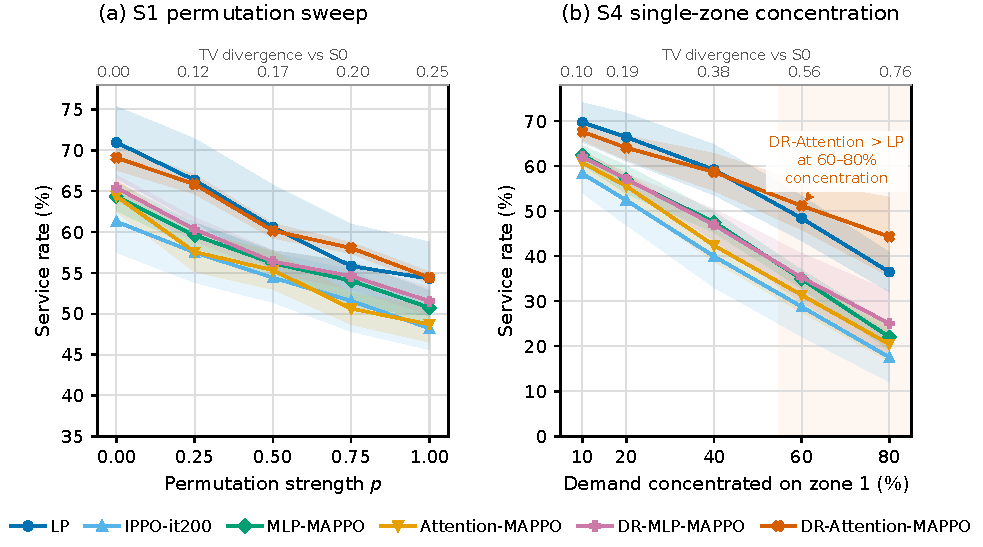
\includegraphics[width=0.59\textwidth]{fig3_parametric_curves.pdf}
\caption{Parametric spatial sweeps, 12 paired windows, bands $\pm1$ std. (a) S1 permutation strength $p$; (b) share of demand concentrated on zone 1. Top axes give TV divergence from S0.}
\label{fig:param}
\end{figure}

Family retention (Fig.~\ref{fig:retention}) summarises the effect. DR-Attention-MAPPO retains $83.8\%$ of its S0 service across the spatial family, against $80.7\%$ for the LP ($+3.1$~pp retention; family-mean service difference $+0.62$~pp, $p=0.37$) and $76.9\%$ for MLP-MAPPO ($+6.9$~pp retention; $+8.44\pm1.70$~pp, $p=2.69\times10^{-9}$). DR raises spatial retention by $9.9$~pp on the attention encoder and not at all on the MLP. On the other families it is level with the LP: $96.1\%$ against $96.3\%$ for volume/burst and $102.1\%$ against $100.5\%$ for temporal shifts.

\begin{figure}[tbp]
\centering
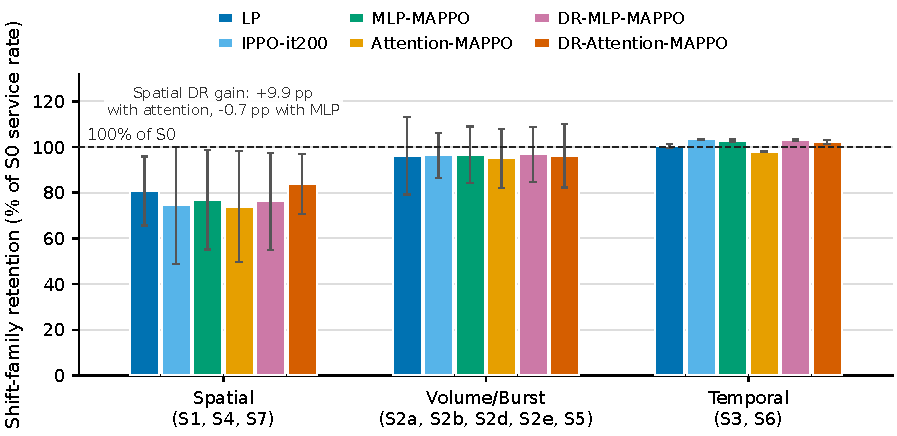
\includegraphics[width=0.52\textwidth]{fig4_retention_2x2.pdf}
\caption{Family retention (service relative to each arm's own S0); error bars $\pm1$ std across scenarios in the family. Families are never pooled.}
\label{fig:retention}
\end{figure}

\section{Limitations}
\label{sec:limitations}

The learned policies are slower to execute: sequential per-zone Python/Torch calls take $5.8$--$7.1$~s per episode against $0.5$~s for the LP. The fleet is small (26 vehicles), speed is constant 30~km/h without congestion, and all sixteen zones are high-volume ($4.84$--$8.29\%$ of training demand), so S4 measures concentration on familiar zones and absolute numbers do not transfer to city scale. Running-maximum normalisation attenuates absolute volume, partly shielding observations from volume shifts. The attention encoder was trained only with MAPPO, and DR covers only permutation and concentration, so unmodelled shifts are untested. The DR-Attention advantage over the LP on S4 is a single concentration family; its spatial-retention edge over the LP is not significant. Averaging RL arms over $n=5$ seeds per window places the paired tests ($n=12$) across demand windows rather than independent seeds, so seed-level sample size limits power for small effects (e.g.\ the S0 Welch test, $p=0.15$). DR-Attention-MAPPO still drives $49$--$100$~km more empty distance than the LP on matched scenarios because the LP solves a coupled multi-zone transportation problem over a smoothed EMA forecast every minute and holds idle cars below its tuned deficit penalty, whereas PPO controllers act myopically every $0.5$~min with entropy regularisation and a fixed $\beta=0.06$ that is not co-tuned like the LP's deficit penalty.

\section{Conclusion}
\label{sec:conclusion}

On NYC16, frozen learned rebalancers hold up under temporal and volume shifts but lose most under spatial shifts. MAPPO beats IPPO on paired windows, mainly by avoiding seed collapse, yet both trail a tuned LP. The gap is not capacity: behaviour cloning the LP into the same network nearly closes it; it comes from optimisation, argmax symmetry and overlong relocation legs. Permutation-equivariant attention and domain randomisation are each insufficient alone, but together match the LP on base, test and permutation demand and exceed it under strong single-zone concentration, at $49$--$100$~km more empty distance (while achieving higher exact reward on S4, $p=0.025$).

\paragraph{Reproducibility}
Code and figures: \url{https://github.com/sharifmdathar/marl-fleet-rebalancing}. Training and evaluation are driven by \path{marl_fleet_rebalancing.experiments.train} and \path{...evaluate} with \texttt{-{}-env nyc}. Checkpoints and evaluation outputs are available on request.

\paragraph{Declaration of generative AI in the writing process}
During the preparation of this work the authors made light use of AI to reformat and draft the text. The authors reviewed and edited the manuscript and take full responsibility for the publication.

\setlength{\bibsep}{2pt plus 0.3ex}
\begin{thebibliography}{24}
\bibitem{xu2018} Z. Xu \emph{et al.} (2018) ``Large-scale order dispatch in on-demand ride-hailing platforms: A learning and planning approach,'' in \emph{Proc. ACM SIGKDD}.
\bibitem{lin2018} K. Lin, R. Zhao, Z. Xu and J. Zhou (2018) ``Efficient large-scale fleet management via multi-agent deep reinforcement learning,'' in \emph{Proc. ACM SIGKDD}.
\bibitem{qin2020} Z. T. Qin \emph{et al.} (2020) ``Ride-hailing order dispatching at DiDi via reinforcement learning,'' \emph{INFORMS Journal on Applied Analytics} 50(5).
\bibitem{oda2018} T. Oda and C. Joe-Wong (2018) ``MOVI: A model-free approach to dynamic fleet management,'' in \emph{Proc. IEEE INFOCOM}.
\bibitem{alabbasi2019} A. O. Al-Abbasi, A. Ghosh and V. Aggarwal (2019) ``DeepPool: Distributed model-free algorithm for ride-sharing using deep reinforcement learning,'' \emph{IEEE Transactions on Intelligent Transportation Systems} 20(12).
\bibitem{holler2019} J. Holler \emph{et al.} (2019) ``Deep reinforcement learning for multi-driver vehicle dispatching and repositioning problem,'' in \emph{Proc. IEEE ICDM}.
\bibitem{li2019} M. Li \emph{et al.} (2019) ``Efficient ridesharing order dispatching with mean field multi-agent reinforcement learning,'' in \emph{Proc. WWW}.
\bibitem{shou2020} Z. Shou and X. Di (2020) ``Reward design for driver repositioning using multi-agent reinforcement learning,'' \emph{Transportation Research Part C: Emerging Technologies} 119.
\bibitem{jiao2021} Y. Jiao \emph{et al.} (2021) ``Real-world ride-hailing vehicle repositioning using deep reinforcement learning,'' \emph{Transportation Research Part C: Emerging Technologies} 130.
\bibitem{gammelli2021} D. Gammelli, K. Yang, J. Harrison, F. Rodrigues, F. C. Pereira and M. Pavone (2021) ``Graph neural network reinforcement learning for autonomous mobility-on-demand systems,'' in \emph{Proc. IEEE CDC}.
\bibitem{guo2021} X. Guo, N. S. Caros and J. Zhao (2021) ``Robust matching-integrated vehicle rebalancing in ride-hailing system with uncertain demand,'' \emph{Transportation Research Part B: Methodological} 150.
\bibitem{schulman2017} J. Schulman, F. Wolski, P. Dhariwal, A. Radford and O. Klimov (2017) ``Proximal policy optimization algorithms,'' arXiv:1707.06347.
\bibitem{pettingzoo} J. K. Terry \emph{et al.} (2021) ``PettingZoo: Gym for multi-agent reinforcement learning,'' arXiv:2009.14471.
\bibitem{yu2022} C. Yu, A. Velu, E. Vinitsky, J. Gao, Y. Wang, A. Bayen and Y. Wu (2022) ``The surprising effectiveness of PPO in cooperative multi-agent games,'' in \emph{Proc. NeurIPS}.
\bibitem{pinto2017} L. Pinto, J. Davidson, R. Sukthankar and A. Gupta (2017) ``Robust adversarial reinforcement learning,'' in \emph{Proc. ICML}.
\bibitem{tobin2017} J. Tobin \emph{et al.} (2017) ``Domain randomization for transferring deep neural networks from simulation to the real world,'' in \emph{Proc. IEEE/RSJ IROS}.
\bibitem{kirk2023} R. Kirk, A. Zhang, E. Grefenstette and T. Rockt\"aschel (2023) ``A survey of generalisation in deep reinforcement learning,'' \emph{Journal of Artificial Intelligence Research} 76.
\bibitem{rashid2018} T. Rashid \emph{et al.} (2018) ``QMIX: Monotonic value function factorisation for deep multi-agent reinforcement learning,'' in \emph{Proc. ICML}.
\bibitem{foerster2018} J. Foerster, G. Farquhar, T. Afouras, N. Nardelli and S. Whiteson (2018) ``Counterfactual multi-agent policy gradients,'' in \emph{Proc. AAAI}.
\bibitem{lowe2017} R. Lowe \emph{et al.} (2017) ``Multi-agent actor-critic for mixed cooperative-competitive environments,'' in \emph{Proc. NeurIPS}.
\bibitem{yang2018} Y. Yang \emph{et al.} (2018) ``Mean field multi-agent reinforcement learning,'' in \emph{Proc. ICML}.
\bibitem{tlc2026} New York City Taxi and Limousine Commission (2026) ``High Volume For-Hire Vehicle Trip Records, April 2026 [data set],'' \url{https://www.nyc.gov/site/tlc/about/tlc-trip-record-data.page}. Accessed 5 November 2026.
\bibitem{vaswani2017} A. Vaswani \emph{et al.} (2017) ``Attention is all you need,'' in \emph{Proc. NeurIPS}.
\bibitem{zaheer2017} M. Zaheer, S. Kottur, S. Ravanbakhsh, B. P\'oczos, R. Salakhutdinov and A. Smola (2017) ``Deep sets,'' in \emph{Proc. NeurIPS}.
\end{thebibliography}

\end{document}
